\section{Layout}

Figure \ref{fig:lay} shows the layout designed for the OTA.

\begin{figure}[!htb]
	\centering
	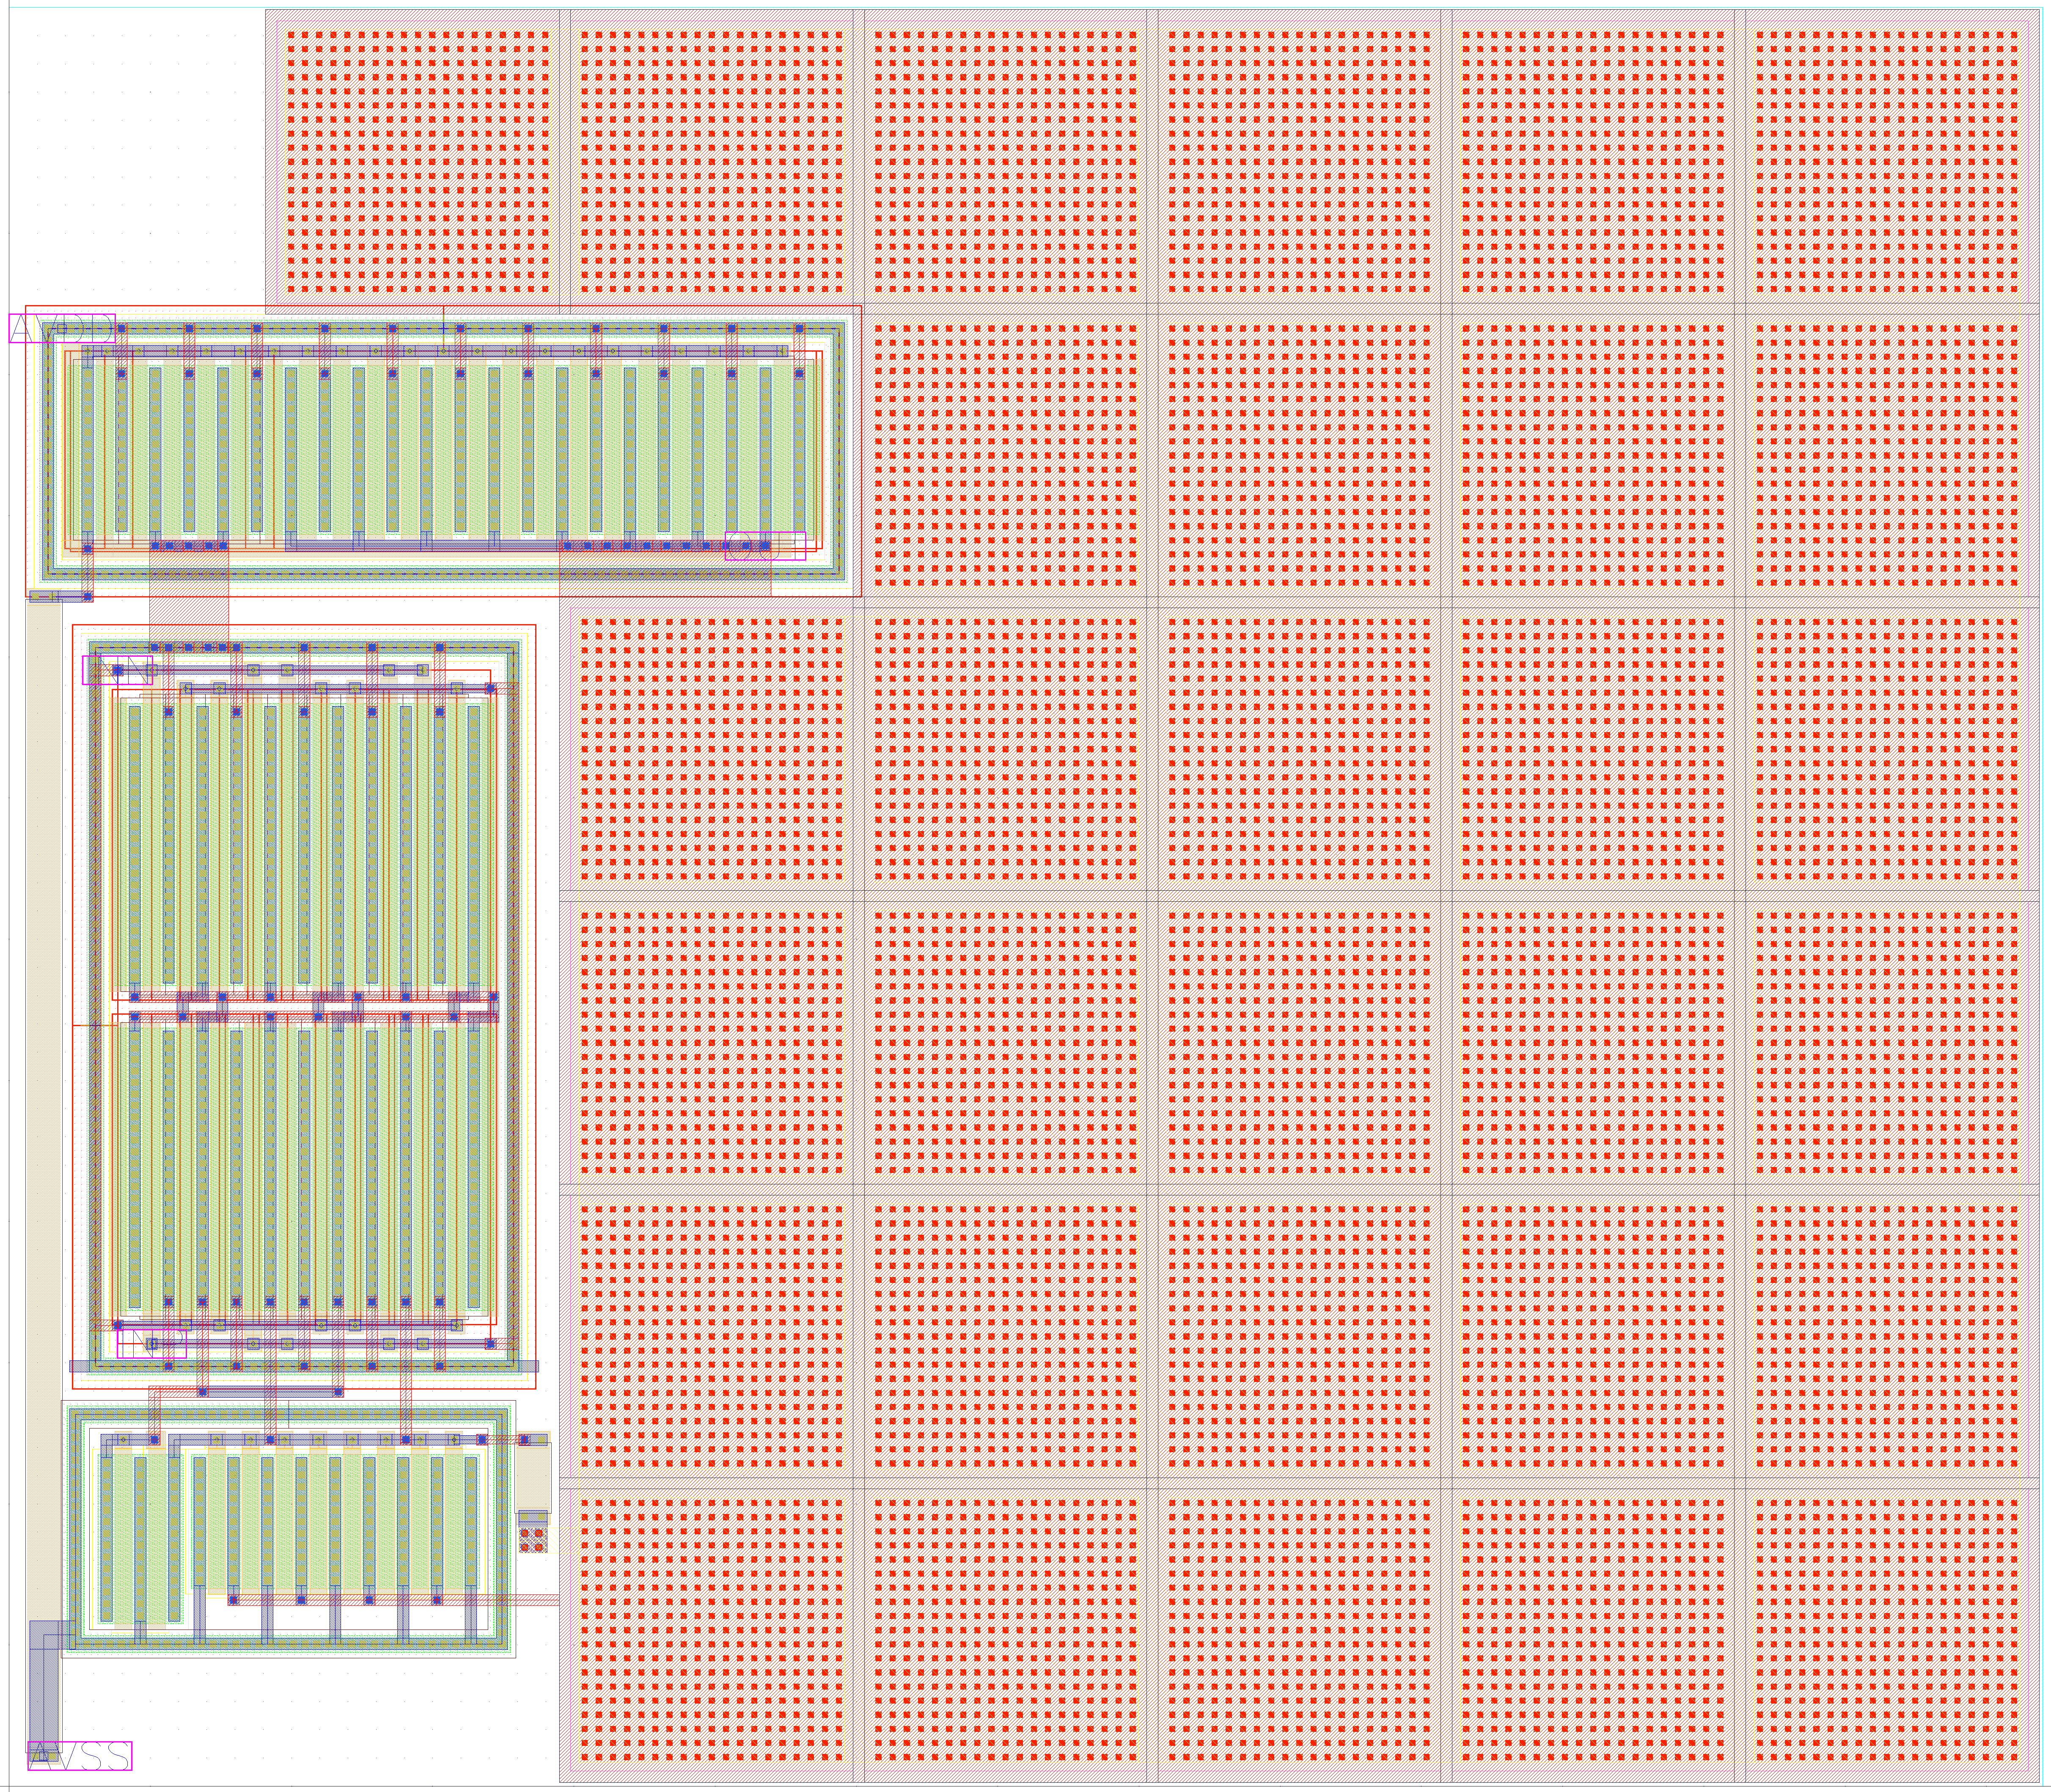
\includegraphics[width=\textwidth]{lay}
	\caption{Layout design of the OTA}
	\label{fig:lay}
\end{figure}

This layout design passed the DRC and LVS verification, as shown in Figure \ref{fig:vfy}.

\begin{figure}[!htb]
	\centering
	\begin{subfigure}[b]{0.5\textwidth}
		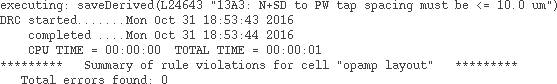
\includegraphics[width=\textwidth]{drc}
		\caption{DRC checking result, no errors}
		\label{fig:drc}
	\end{subfigure}
	\begin{subfigure}[b]{0.4\textwidth}
		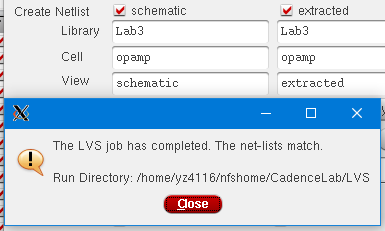
\includegraphics[width=\textwidth]{lvs}
		\caption{LVS checking result, the extracted net-list matches the schematic}
		\label{fig:lvs}
	\end{subfigure}
	\caption{Layout design verification}
	\label{fig:vfy}
\end{figure}

For better device matching, the PMOS transistors PM0 and PM1 from differential pair were placed closer together, using common centroid layout technique, as shown in Figure \ref{fig:ltp}. These 2 MOSFETs were split to 10 smaller transistors each, represented by the red and green boxes respectively.

\begin{figure}[!htb]
	\centering
	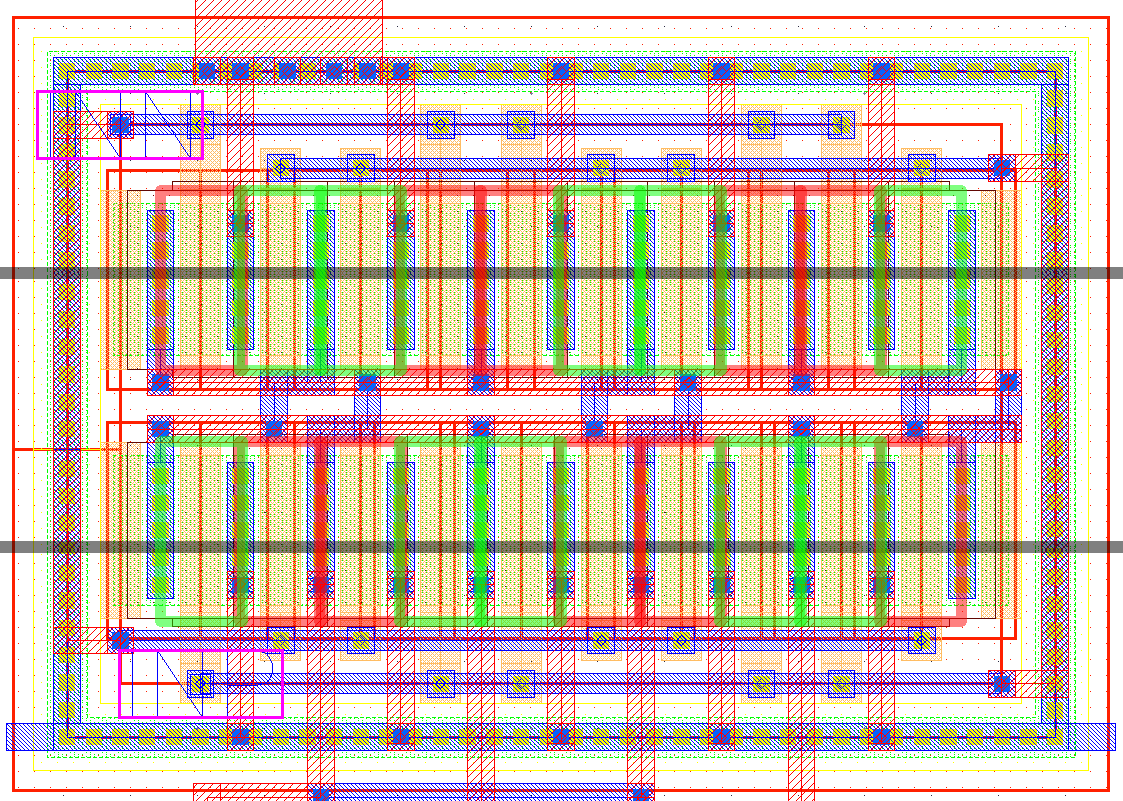
\includegraphics[width=0.8\textwidth]{ltp}
	\caption{Layout of the LTP, vertically shrunk along the black lines}
	\label{fig:ltp}
\end{figure}

4 dummy poly silicon gates including active area were added to the edges of the LTP. These reduce the edge effect due to etching, improves device matching.

The current mirror PM5, PM2 and PM4 were placed together and implemented using a base width of $6\mu m$, and multiple fingers for multiplication. This gives better multiplication ratio with identical unit devices. Figure \ref{fig:cm} shows the layout details of the current mirror. Dummy poly silicon gates were also added to reduce edge effect.

\begin{figure}[!htb]
	\centering
	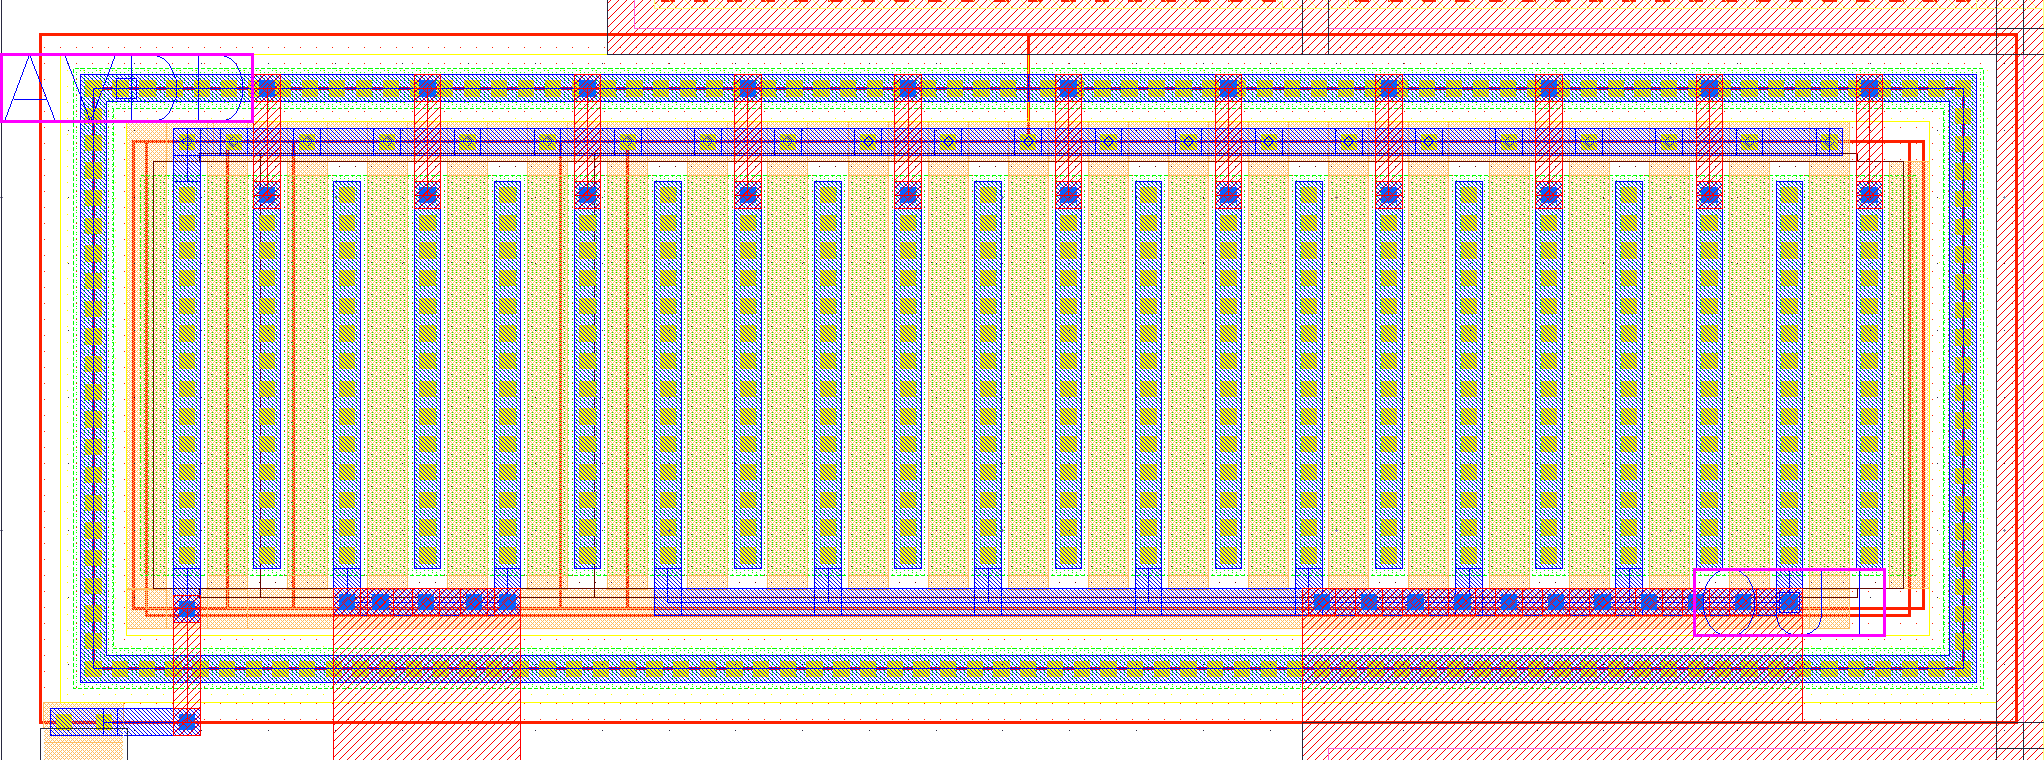
\includegraphics[width=\textwidth]{cm}
	\caption{Layout of the PMOS current mirror}
	\label{fig:cm}
\end{figure}

NM3 from amplification stage was also split into multiple fingers, to reduce parasitic resistances and capacitances.
